\documentclass[11pt,a4paper,oneside]{article}
\usepackage[T1]{fontenc}
\usepackage[utf8]{inputenc}
\usepackage[french,english]{babel}
\usepackage[babel=true,kerning=true]{microtype}
\usepackage[usenames,dvipsnames,svgnames,table]{xcolor}
\usepackage[colorlinks,linkcolor={blue!30!black},citecolor={blue!50!black},urlcolor={blue!80!black}]{hyperref}
\usepackage{amsmath,amsfonts,amssymb,array,graphicx,caption,lmodern,subcaption,tikz,url,xspace,wrapfig}
\usepackage{textcomp,rotating,epic,eepic,pdfpages,listings,diagbox,multirow,float}

\usepackage[top=20mm,bottom=20mm,left=25mm,right=25mm]{geometry}
%\usepackage[top=15mm,bottom=15mm,left=15mm,right=15mm]{geometry}

\parskip=6pt % adds vertical space between paragraphs

\DeclareMathOperator{\e}{e}

\begin{document}

\pagenumbering{gobble}  % Pas de numérotation
\begin{titlepage}
    \vspace*{50px}
    
\includegraphics[height=80px]{Images/logo_phelma.pdf}
    \vspace*{-80px}
\begin{flushright}
%     \vspace*{60px}
    
\includegraphics[height=65px]{Images/CIME.jpg}
\end{flushright}

\vspace*{2cm}

\begin{center}
\rule{\linewidth}{0.5mm}\\[0.4cm]
{\huge{\bfseries Compte Rendu}\\[0.4cm]
\textsc{TP Simulation électronique}\\[0.4cm]}
\rule{\linewidth}{0.5mm}\\[0.5cm]

\LARGE{\textsc{Nicolas Paillet, Félix Piédallu \& Giulia Rizzo}}\\[0.7cm]
\large{\textsc{2015-2016}}\\[2cm]

\Large{~}\\[1cm]
% 
\includegraphics[width=0.4\textwidth]{Images/CIME.jpg}\\[1cm]
%
 \large{Encadrant : Marco Pala}\\[2cm]
%

\end{center}
\end{titlepage}

\tableofcontents        % Table des matières avec liens, générée automatiquement.
\newpage
\pagenumbering{arabic}  % Numérotation de retour !


\section*{Introduction}
\addcontentsline{toc}{section}{Introduction}
	
		
Extended X-ray Absorption Fine Structure (EXAFS) is a spectroscopic method to caracterize elements of a sample (fluid or solid). The sample is placed on the trajectory of a X-ray beam, insensity of the X-ray is mesured before and after the sample, it give us absorption of the X-ray produced by passing through the sample.\\
 The sample is scanned by X-rays of differents energies. In the EXAFS domain, kinetic enregy of photoelectron sent is from 50 eV to 1000 eV approximatively.\medskip
	 
 This study is composed of two parts: Firstly, we are going to devellop theorical aspects of the EXAFS and working principle of the CERN used. Secondly, how to make standards samples and exploitations of results.
	



\newpage
	

\section{Theorical aspects}
\subsection{EXAFS Domain and utilisation}


\subsection{Grenoble CERN Operating principle}

The Hall where all experiments lines are regrouped is in the figure \ref{Hall}.\medskip

\begin{figure}[H]
    \begin{center}
        %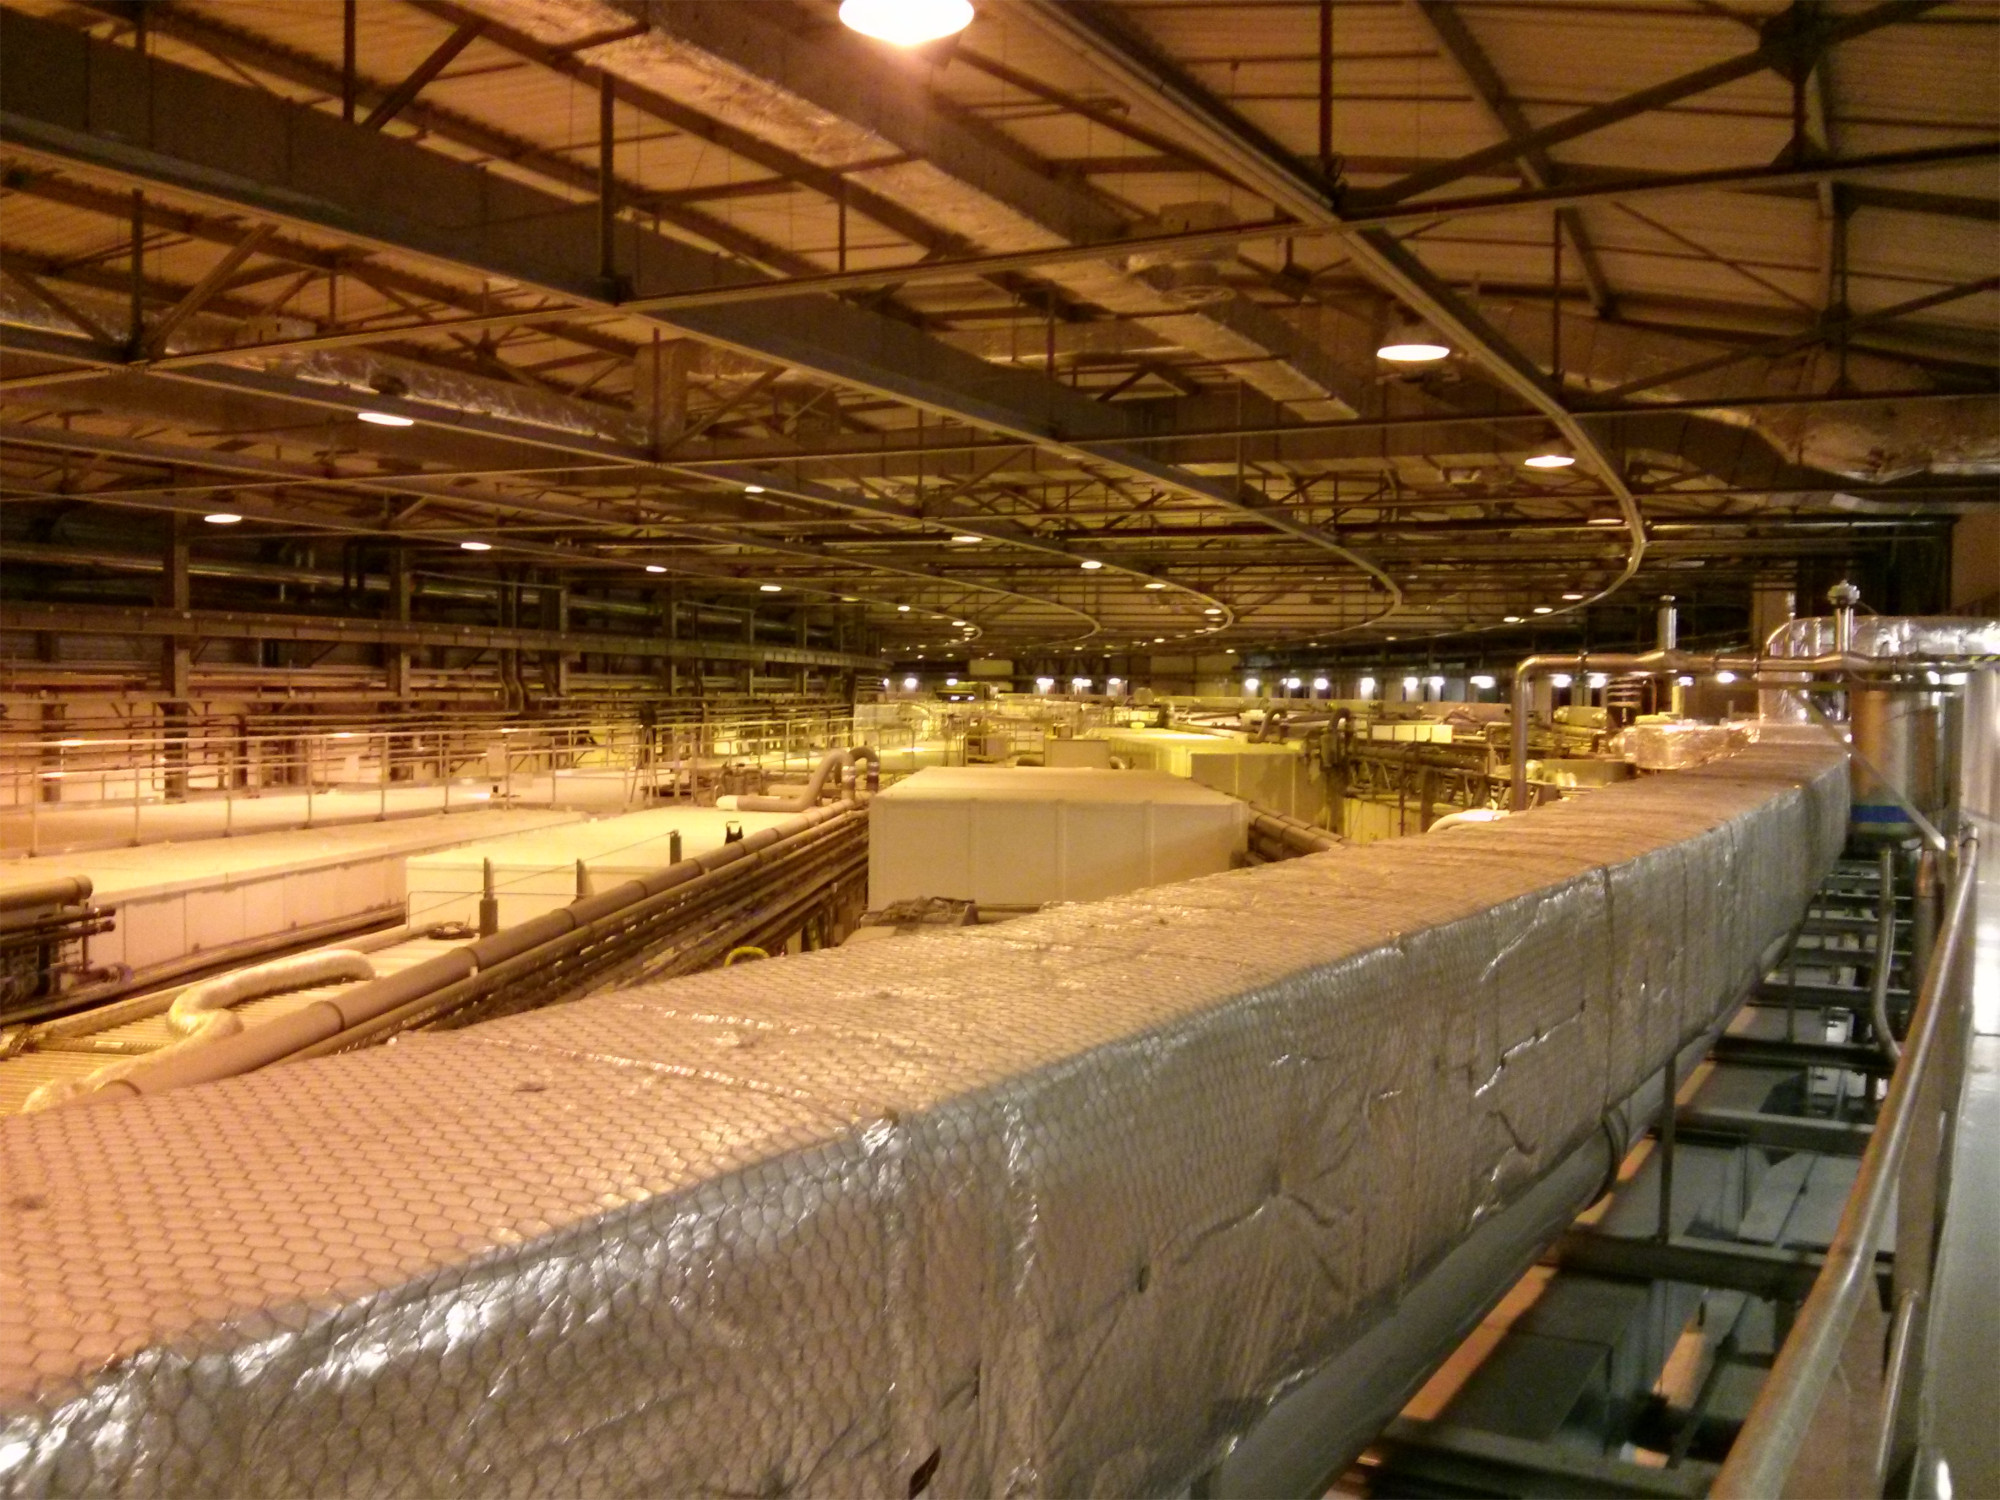
\includegraphics[scale=0.15]{Images/IMG_20151210_213319.jpg}
        \caption{Hall of experiments (CERN Grenoble)}
        \label{Hall}
    \end{center}
\end{figure}
\medskip



\newpage



\section{Experimental measurements}
\subsection{Reference sample Cu foil}


\subsection{Cu2O sample construction}


\subsection{Graph analysis and results} \label{results}


\subsubsection{Absorption graph}


\subsubsection{Neighbours distance graph}

 
\newpage

\section*{Conclusion}
\addcontentsline{toc}{section}{Conclusion}

Au cours de cette étude, nous avons pu mettre en évidence


\nocite{*}
\bibliographystyle{unsrt}
\bibliography{Biblio}
\end{document}
